\section{Convolution}
This section introduces the convolution from a more mathematical perspective and then gives some less traditional applications of a more generalized version.

\subsection{Definition}
Conceptually, the convolution operation gives the overlap between two functions as a function of the offset between the functions.

Mathematically, convolution is defined by an integral:

\[
    (f * g)(t) = \int^{\infty}_{-\infty}{f(\tau)g(t-\tau) d\tau}
\]

Its discrete counterpart is:

\[
    (f * g)(n) = \sum^{\infty}_{i=-\infty}{f(i)g(n-i)}
\]

\begin{figure}
    \centering
    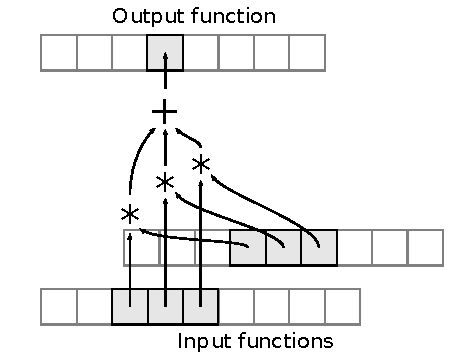
\includegraphics{img/VisualConvolution}
    \caption{
        Convolution performed on discrete functions.
        Each box represent an output value of the function.
    }
    \label{fig:VisualConvolution}
\end{figure}

This is visualized in figure \ref{fig:VisualConvolution} where we have focused on only 3 of the values in the input functions. Notice how the corresponding values from the input functions are multiplied together before the products are summed.

This can also be extended to multiple dimensions by summing across the additional dimensions.
For the discrete case, this gives
\[
    (f * g)(n, m) = \sum^{\infty}_{i=-\infty}\sum^{\infty}_{j=-\infty}{f(i, j)g(n-i, m-j)}
\]

\subsection{Application in Image Processing}
As mentioned in the introduction, convolution can be used in image processing to apply various filters to an image.

A monochrome image can be thought of as a 2D matrix with a width $W$ and height $H$.
Let $I(x, y)$ be a function for accessing a specific value in the image matrix.
Let $K(x, y)$ be a function for accessing a specific value in a special matrix called the \textit{kernel},
or $0$ if $x$ or $y$ is out of bounds for the matrix.

The convolution of the image and the kernel is then given by
\[
    C(x, y) = \sum^{H}_{h=0} \sum^{W}_{w=0}{I(w, h)K(w - x, h -y)}
\]
where $C(x, y)$ is the output image.

For a coloured image, each channel is processed separately.

Depending on the kernel matrix, various effects like blurring or sharpening may be applied to the image with convolution.
A small selection of possible kernel matrices and the results the produce can be found in table \ref{tab:KernelMatrices}.

\begin{table}
    \begin{tabular}{ccm{2cm}}
    Description & Matrix & Result \\
    \hline
    Blur & $
            \begin{bmatrix}
            1/9 & 1/9 & 1/9 \\
            1/9 & 1/9 & 1/9 \\
            1/9 & 1/9 & 1/9
            \end{bmatrix}
        $ & 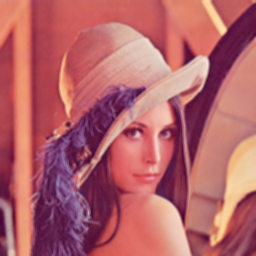
\includegraphics[width=2cm]{img/LenaBlurred} \\
    Edge-detect & $
            \begin{bmatrix}
            -1 & -1 & -1 \\
            -1 & 8 & -1 \\
            -1 & -1 & -1
            \end{bmatrix}
        $ & 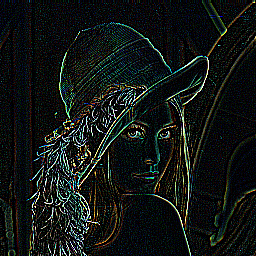
\includegraphics[width=2cm]{img/LenaEdge} \\
    Emboss & $
            \begin{bmatrix}
            -2 & -1 & 0 \\
            -1 & 1 & 1 \\
            0 & 1 & 2
            \end{bmatrix}
        $ & 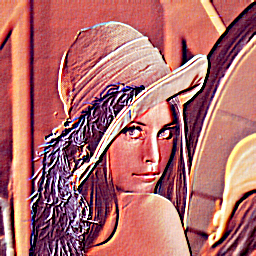
\includegraphics[width=2cm]{img/LenaEmbossed}
    \end{tabular}
    \caption{Some kernels used in image processing}
    \label{fig:KernelMatrices}
\end{table}

As the matrices in table \ref{tab:KernelMatrices} are good examples of, the kernel matrices used for image processing is usually small compared to the images, and often of a constant size.
This means each output pixel is a function of the same pixel in the original image and its neighbourhood.

\subsection{Generalized convolution}
We can abstract the convolution process by using mapping function $f: R x R \rightarrow R$ in place of multiplication, and $g: R x R \rightarrow R$ in place of addition.
A convolution can then be described as $(f, g)$, from here on referred to as the map function and the reduce function, where the standard convolution can be expressed whit $(*, +)$, while $(min, +)$ describes finding the shortest path.
The only restriction we impose on $f$ and $g$ is that they form a semiring.
Abstract algebra is outside of the scope of our report, but informally we impose that the TODO 

Can we use domains outside of R? 
Describe associativity, for instance show minus not nescessarily working?

\section{Implementing convolution}
On modern computers the memory bandwidth will usually be the bottleneck of any operation involving large amounts of data, such as an image. TODO reference (or is it considered common knowledge?)
The essence of implementing efficient convolution is therefore removing redundant data movement.
Whenever we move a pixel into working memory we ideally want to perform a map operation for every neighbourhood it is part of.
If a pixel is ejected from memory it will have to be retrieved again until all convolutions it is part of has been calculated.
Ideally we would have enough memory to store an entire image and work on all parts simultaneously. While this can certainly be done, if we want speed we have to sacrifice memory size.
The challenge is therefore to use as little memory as possible balanced with reducing redundant loads.\\

